\chapter{基于多源头的主题标签流行度预测}\label{chap:four}

在第三章中,我们介绍了宏观角度的 Hashtag 流行度预测方法,主要是使用 机器学习的方法,人工构造有效特征来进行预测,该方法的好坏很大程度上取决 于人工构造的特征的质量。通过对大多数的 Hashtag 流行度预测案例来看,基于 特征的 Hashtag 流行度预测需要一下几个条件:足够的观测时间窗又,通过大量 观测时间窗又内的数据获取有效的宏观特征;另外需要 Hashtag 本身具有足够的 传播规模。而这些约束条件在某些预测场景下并不满足,而微观视角是从理解传 播过程入手,建模参与用户与传播环境的反馈以及对最终流行度的影响,因此更 适宜解决宏观视角所不能解决的情况。另外基于生成式的消息建模方法不是预 测未来的流行度,因此预测性能是有缺失的。另外消息流行度预测问题解决的是 单源头问题,因此对于多源的 Hashtag 流行度预测建模是目前的研究方向。

针对以上问题,本章提出了一种建模多源 Hashtag 流行度预测的模型,该模 型既可以有效学习每个源头内部的传播方式,又可以通过 attention 机制考虑不 同源头之间的影响,从而刻画整体模型的传播机制。然后使用 TensorFlow 平台 进行了模型训练和测试,通过实验证明了模型的有效性。
\section{问题描述和基本思路}
\subsection{问题描述和基本思路}
目前社交网络中的消息流行度预测都是单源头的问题,每条消息只有一个 源头。此类模型主要是建模从该单一消息源头转发的路径关系。然而,目前常 见的消息流行度预测方法无法很好的建模 Hashtag 流行度预测问题。因为对于同 一个 Hashtag,它可以在不同时刻由不同的用户发出,它的源头不是唯一的,如 何很好的刻画多源头之间的关系是十分必要的。因为对于同一个 Hashtag,当微 博上的一个大 V 用户发出,它的转发量很可能是暴涨的,而对于一个普通用户 发出的,它的转发量可能是很稀少的, 如图4.1所示,重要节点的转发关系是庞大 的,因此刻画每个源头的重要性是十分必要的。另一方面,还需考虑每个源头之 间的传播方式,单独建模好每一个源头的数据对于整体的效果也是十分重要的。 综合考虑这两种方式的优缺点,本章提出了一种既建模了单个源头序列之间的 传播关系又考虑了多个源头之间关系的模型。

为了更好的刻画 Hashtag 传播过程中的机制,本章进行小时级别的数据划分,当一个 Hashtag 由一个源头发出以后 1 小时,分析该 Hashtag 未来 24 小时内 的转发数量。

\begin{figure}[H]
    \centering
    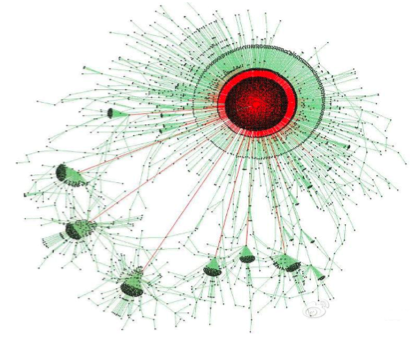
\includegraphics[width=0.5\textwidth]{hashtag_19}
    \bicaption{消息传播方式}{Message dissemination}
    \label{fig:4_2}
\end{figure}

\subsection{基本思路}


目前现有的 Hashtag 流行度预测基本都是基于特征的方法,没有建模它们内 部的传播机制,同时微博消息的流行度预测算法虽然很好的建模了消息的内部 传播机制,但是无法很好的适用到多源头 Hashtag 的流行度预测问题上。为了建 模多源头 Hashtag 流行度预测问题,可以借助算法中的分而治之的思想,既要很 好的建模每一个源头上的消息传播机制,又很好的将每个源头的数据融合在一 起,从而在整体上刻画 Hashtag 的流行度预测模型。

因此,本章的基本思路是首先根据消息传播机制的方式建模 Hashtag 每一个 源头中消息的转发情况,然后对于每一个源头的传播路径得到一个高维表达,通 过 attention 机制衡量每一个源头的重要性,来建模整体的 Hashtag 流行度预测过 程。

\section{相关工作}
由于本文的主要建模办法是采用 attention 机制来刻画 Hashtag 不同源头之间 的重要性,所以首先介绍一下 attention 的基本原理,然后介绍一种刻画消息内部 传播机制的模型,便于后续模型的提出。
\subsection{attention 机制}

Attention 模型最初主要是应用于图像识别中,它主要是模仿当人观看一副 图像时,视线的焦点在物体上的移动。当模型对图像或语言进行识别时,每次集 中于部分重要特征上,识别更加准确。现在在很多自然语言处理的任务上应用也 很多,比如文本分类中,用 attention 来衡量不同词的重要性。然而如何衡量特征 的重要性呢,最直观的方法就是考虑每个特征的权重,因此,Attention 模型的结 果就是在每次识别时,首先计算每个特征的权重,然后对特征进行加权求和,权 值越大,该特征对当前模型的贡献就越大,自动选取到了重要的特征。

机器翻译中的 Attention 模型最直观\citep{Luong2015Effective},并且易于理解,每当生成一个单 词时,找到源句子中与其对应的单词,翻译才准确。此处就以机器翻译为例来讲 解 Attention 模型的基本原理,在介绍 Attention 模型之前,需要先介绍一下机器 翻译领域应用最广泛的模型——Encoder-Decoder(编码-解码)结构 \citep{Bahdanau2014Neural}。

Encoder-Decoder 框架包括两个步骤,第一步是 Encoder(编码),将输入数据 (如图像或文本)编码为一系列特征,第二步是 Decoder(解码),以编码的特征作 为输入,将其解码为目标输出。Encoder 和 Decoder 是两个独立的模型,可以采 用神经网络,也可以采用其他模型进行训练。机器翻译中的 Encoder-Decoder 示
例如图\ref{fig:4_3}所示。该示例将一个句子(ABC)翻译为另一种语言的句子(WXYZ), 其中 A、B、C 和 W、X、Y、Z 分别表示一个字或一个单词,图中每个方框表示 一个循环神经网络模型,不同的方框表示不同时刻的表达,<EOS> 表示句子的 结束。


\begin{figure}[H]
    \centering
    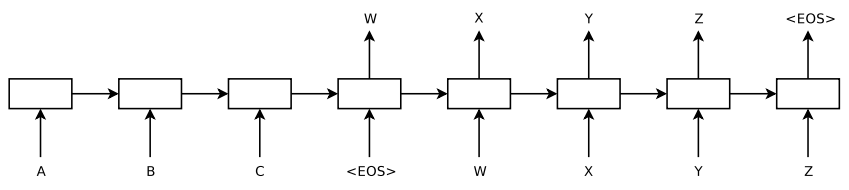
\includegraphics[width=0.5\textwidth]{hashtag_20}
    \bicaption{编码-解码}{Encoder-Decoder}
    \label{fig:4_3}
\end{figure}


Attention 机制在 Encoder-Decoder 中介于 Encoder 和 Decoder 中间,首先根 据 Encoder 的特征计算权值,然后对 Encoder 的特征进行加权求和,作为 Decoder 的输入,其作用是将 Encoder 的特征以更好的方式呈献给 Decoder,找到每个词 对应的重要输入,更好的反映编码与解码之间的关系, 模型如图\ref{fig:4_4}所示,图中的 $a_{t,i}$,i 就是 Attention 模型生成的权值。

\begin{figure}[H]
    \centering
    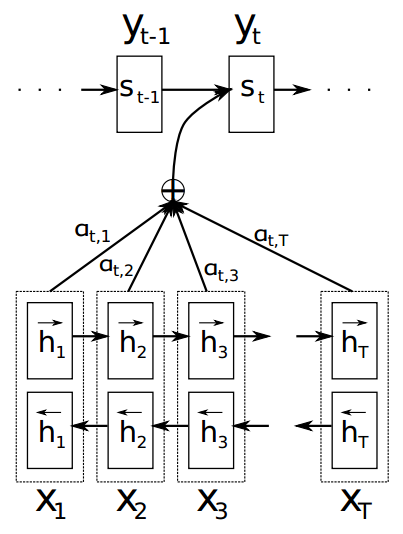
\includegraphics[width=0.5\textwidth]{hashtag_21}
    \bicaption{基于注意力的编码解码过程\citep{Bahdanau2014Neural}}{Attention-based encoder and decoder process\citep{Bahdanau2014Neural}}
    \label{fig:4_4}
\end{figure}

在 t 时刻,对特征 $h $进行加权组合,那么生成新的单词的过程如公式\ref{eq:4_1}所 示, 这里的 $f\_{att}$ 才是 Attention 模型的核心,可以用来估计位置 i 附近的输入和位 置 t 的输出之间的匹配程度,它的表达是不唯一的,常见的是使用一个神经网络 来进行拟合。

\begin{equation}\label{eq:4_1}
	\begin{cases}
	c_t = \sum_{i=1}^T a_{t,i}h_i \\
	a_{t,i} = \frac{\exp(e_{t,i})}{\sum_{k=1}^T \exp(e_t,k)} \\
	e_{t,i} = f_{att}(s_{t-1},h_i)\\
	f_{att}(s_{t-1},h_i) = \tanh(W_as_{t-1} + U_ah_i)
	\end{cases}
\end{equation}

\subsection{DeepHawkes 模型}


在第二章的相关工作中,本文已经详细介绍过了 DeepHawkes 模型 \citep{Cao2017DeepHawkes},它 使用神经网络进行消息流行度预测,该模型既可以建模消息的内部传播机制,又 将消息的未来流行度作为目标进行预测,是目前不错的消息流行度预测模型。但 是在其建模消息传播机制中的时间衰减影响的时候,该模型学习到的是一个固 定结果, 如图\ref{fig:4_5}所示,认为所有的数据在相同时刻的影响力是一样的。但是实际
 上相同时间段内的数据由于不同的传播路径,不同的路径长度等因素,导致它们 的影响力是不同的,因此本文对其进行改进,使用 attention 来刻画每个过程的影 响,既考虑时间衰减的影响又加上传播路径的信息,更加全面的刻画不同路径的 权重。
\begin{figure}[H]
    \centering
    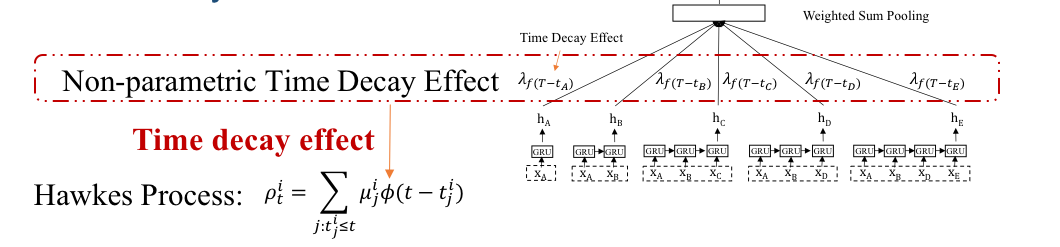
\includegraphics[width=1\textwidth]{hashtag_22}
    \bicaption{DeepHawkes 模型中的时间衰减影响\citep{Cao2017DeepHawkes}}{Time Decay Effect in DeepHawkes Model\citep{Cao2017DeepHawkes}}
    \label{fig:4_5}
\end{figure}

\section{多源 Hashtag 流行度预测模型}
考虑到消息传播中的单源传播模型无法很好的刻画多源 Hashtag 流行度预
测问题,结合 attention 机制,本章提出了一种多源 Hashtag 流行度预测模型。
\subsection{模型结构}

本章提出了一种基于 attention 的多源头 Hashtag 流行度预测模型。模型的结 构如图\ref{fig:4_6}所示, 主要由以下几部分组成:

\begin{enumerate}
\item 首先通过 LINE,将用户网络粉丝结构生成每个用户的向量表达,作为传 播路径上的每个用户的输入;
\item 然后将Hashtag传播路径进行编码,通过循环神经网络进行建模,刻画每 个源头上 Hashtag 的传播机制;
\item 通过考虑序列间的 attention 机制,刻画相同源头上 Hashtag 不同传播路 径的影响力;
\item 通过考虑不同源头的 attention 机制,刻画每一个 Hashtag 源头对于整体 Hashtag 流行度的影响;
\item 最后通过神经网络全连接来预测目标值。

\end{enumerate}

\begin{figure}[H]
    \centering
    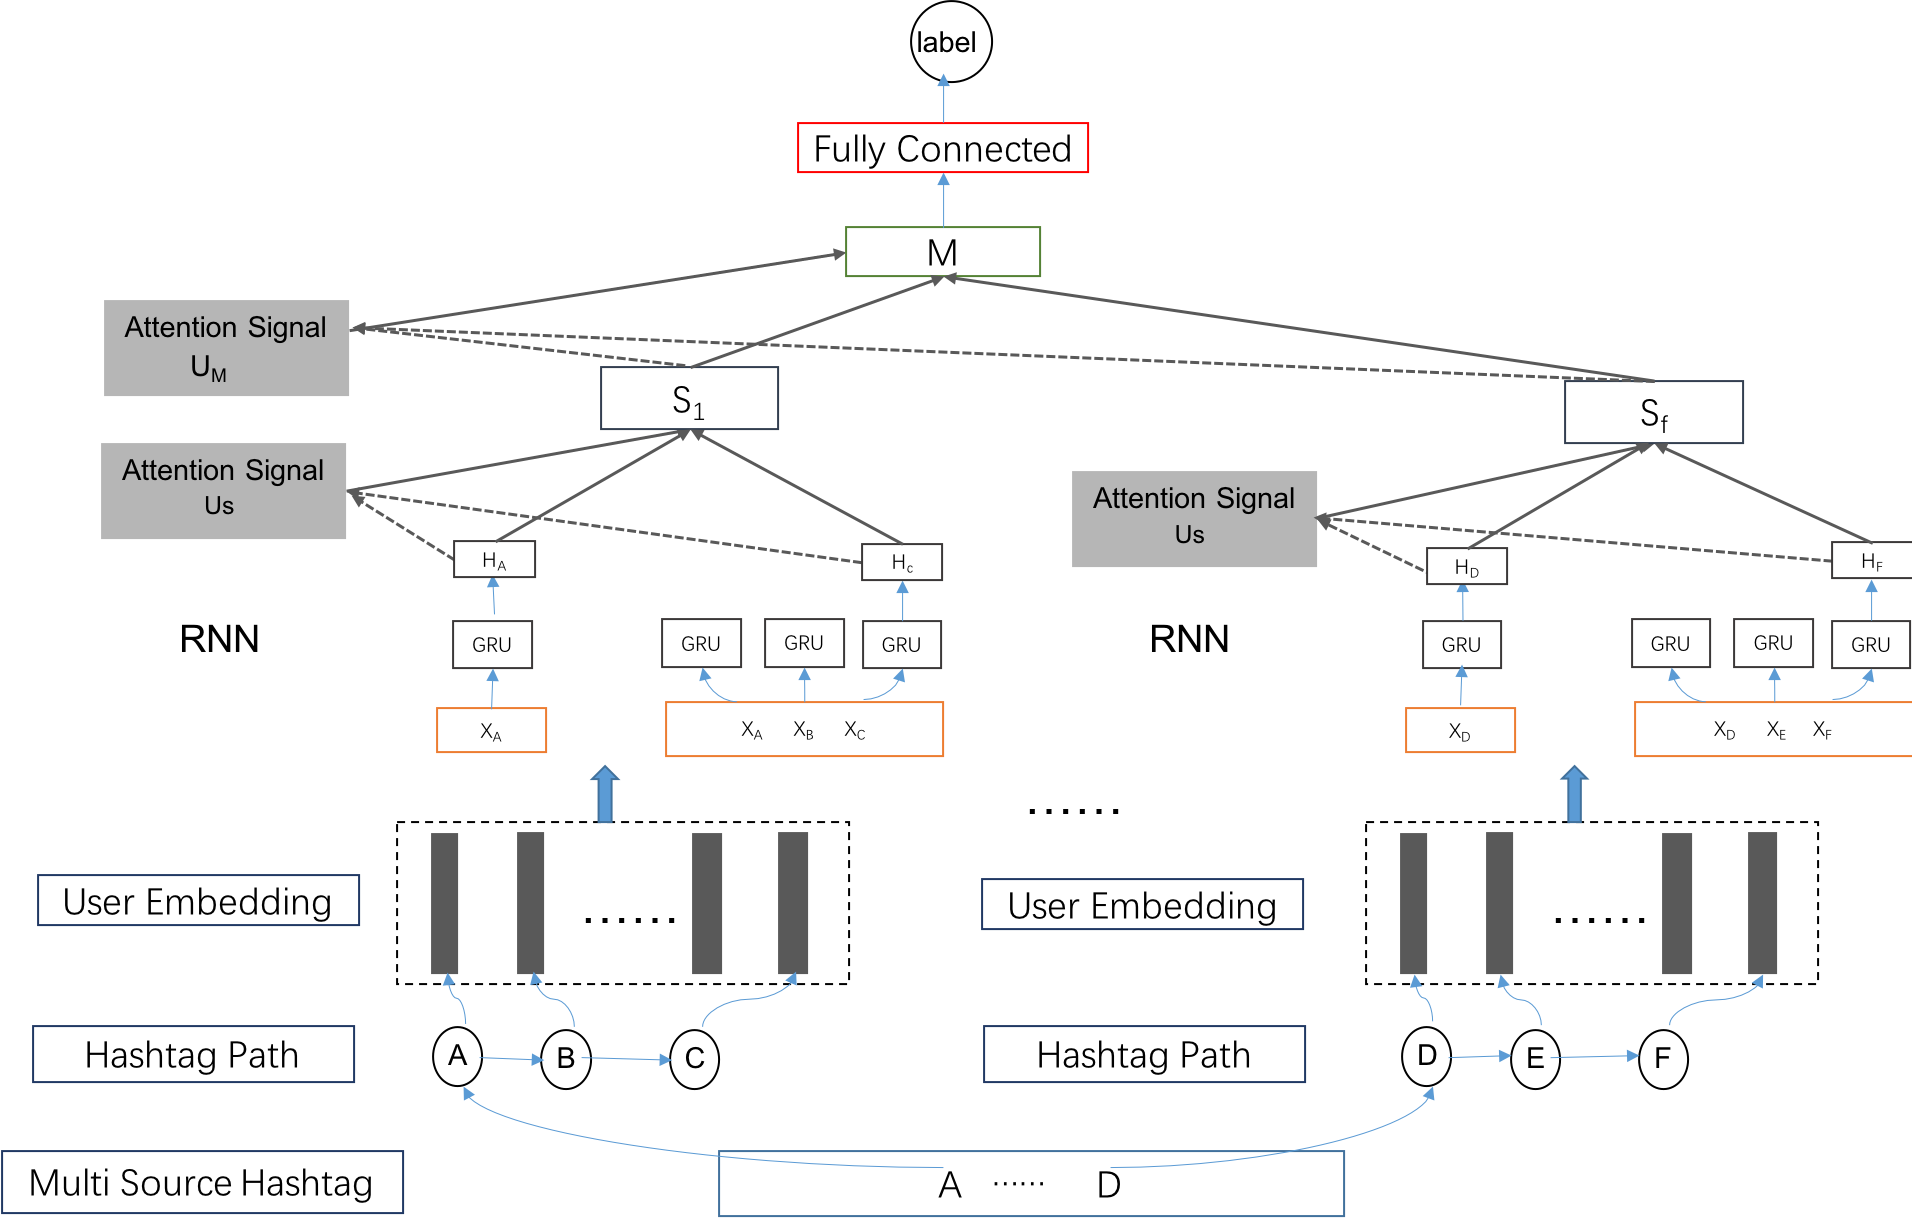
\includegraphics[width=1\textwidth]{model}
    \bicaption{基于注意力的多源 Hashtag 流行度预测}{Multi-source Hashtag popularity prediction based on attention}
    \label{fig:4_6}
\end{figure}

与传统的 Hashtag 流行度预测模型相比,本章提出的模型有如下几个创新 点:
\begin{enumerate}
\item 之前的 Hashtag 流行度预测都是基于特征的方式,本文第一次采用神经 网络建模主题标签的传播方式,便于理解影响 Hashtag 流行度的因素;
\item 对于传统的消息时间衰减影响,本文采用 attention 机制进行学习,有效 刻画每个元素的影响;
\item 本文对于多源头的 Hashtag 进行建模,通过 attention 机制刻画不同源头 的重要性。

\end{enumerate}

\subsection{User Embedding Layer}
User Embedding Layer 把每一个用户映射成一个分布式向量表示,user embedding 有两个好处,第一个是可以自动学习用户的分布式表示,第二个好处是 可以大大缩小参数空间,加快训练速度。在这里,本文使用了预训练的方式,首 先,使用 LINE 模型根据用户粉丝网络结构进行用户分布式学习,得到网络结构 中每个用户的分布式表示,作为模型里面出现的用户的初始化表示,这样通过 加入先验知识的方式可以提高模型的训练速度,同时减少过拟合,将用户向量 刻画的更细致;并且根据第三章的内容可以得知用户的粉丝网络结构特征对于Hashtag 流行度预测是有一定作用的,因此可以提高模型的效果。

\subsection{RNN Layer}

对于 Hashtag 多源头中的每一个源头消息,较好的刻画其具体传播特性对于 整体的预测效果是十分重要的。在转发过程中,每一次的转发都可能改变未来转 发的情况,在实际情况中,不仅当前转发用户本身对于未来转发有影响,而整个 转发路径也会有所贡献。因此,本层不仅仅对当前转发用户进行建模,而是通过 递归神经网络对整个转发路径进行编码。这种做法主要是出于两点考虑:一个 是影响的传递性,以前的参与者不仅影响其直接转发者,而且通过转发方式对 间接转发者产生影响,因此整个转发路径上的每个用户都会对后续转发产生影 响;另一个是结构位置信息,通过用户在转发路径上出现的次数来表征,来衡量 用户的重要性,如图\ref{fig:cascade}所示, 节点 B 在整个消息传播过程中是十分重要的,总之 该层主要是对整个转发路径进行建模。通过以上分析,因此本层使用 GRU,一 种 RNN 的变形体进行序列建模,对于每个序列输入 [$X_{A},X_{B},X_{C}...X_{N}$], 通过 GRU 得到得到每一序列的输出$H_{A}$, 公式如\ref{eq:4_1_g}所示。由于每个序列的长度是不固定的, 因此对于每个序列的输出,本文选取最后一个实际的节点作为循环神经的输出, 这样考虑了数据的有效性。

\begin{equation}\label{eq:4_1_g}
H_A = GRU([X_A,X_B,X_C...X_N])
\end{equation}

\begin{figure}[H]
    \centering
    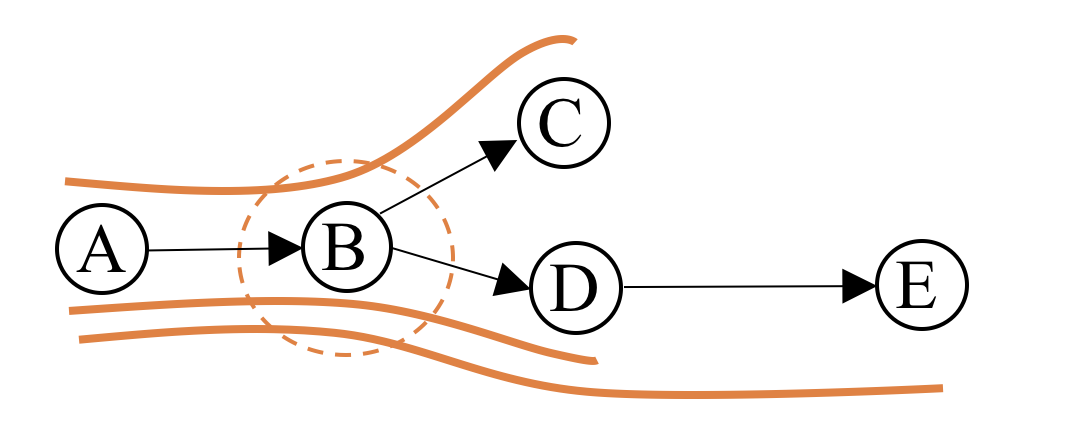
\includegraphics[width=0.8\textwidth]{cascade}
    \bicaption{消息级联传播展示图}{Message cascade display}
    \label{fig:cascade}
\end{figure}

\subsection{第一层 attention}
已有的研究证明了时间衰减对消息传播的影响,但是传统的方式都是需要 建模时间衰减函数,然而在不同的领域,这个函数很可能是不一样,因此很难建 模。为了避免以上问题,因此本文采用 attention 机制,考虑每个序列的 GRU 输出以及此时刻的时间因素,自动学习每个序列的时间衰减影响,最终的结果输出 $S_{i}$如公式\ref{eq:4_1_a}所示。公式里面的$H_{it}$表示上一层的序列输出,$T_{it}$表示该序列的时 间间隔因素,$U_{S}$ 表示 attention 的上下文向量,是一个高维向量表示,这个向量 通过随机初始化得到,并不断学习,$S_{i}$ 表示 attention 层的输出。

\begin{equation}\label{eq:4_1_a}
	\begin{cases}
	u_{it} = \tanh(W_S(H_{it}+T_{it}) +b_S)\\
	\alpha_{it} = \frac{\exp(u_{it}U_S)}{\sum_{t} \exp(u_{it}U_S)} \\
	S_i = \sum_{t}\alpha_{it} H_{it}
	\end{cases}
\end{equation}

\subsection{第二层 attention}

对于多源头的 Hashtag 流行度预测,由于每个源头的重要性是不同的,如何 衡量它们之间的重要性和区分度是本研究的难题。为了更好的刻画每个源头的 重要性,本文采用 attention 机制,对于每一个源头计算一个权重,然后求得最终 的结果,公式如\ref{eq:4_2_a}所示,公式中的 $S_{i}$ 表示每个源头的向量表达,$U_{M}$是一个源 头级别的上下文向量, 该向量通过随机初始化然后不断学习,向量 M 表示最后的 多源头向量的整合。

\begin{equation}\label{eq:4_2_a}
	\begin{cases}
	u_i = \tanh(W_mS_i +b_m)\\
	a_i = \frac{\exp(u_iU_M)}{\sum_{i} \exp(u_iU_M)} \\
	M = \sum_{i}\alpha_i S_i
	\end{cases}
\end{equation}

\subsection{全连接层}
模型的最后一层是多层感知机,通过将上一层 attention 的输出 M 作为本层
 的输入,本层的输出直接是最终的目标,公式如\ref{eq:m_1}所示:

\begin{equation}\label{eq:m_1}
Label = MLP(M)
\end{equation}
模型的最小化的目标函数如\ref{eq:o_1}所示:


\begin{equation}\label{eq:o_1}
obj = \frac{1}{N}\sum_{i=1}^N(\log Prediction - \log Label)^2
\end{equation}

公式里面的N表示全部的Hashtag的数量,prediction代表预测值,label表示真实值,通过取对数的方式可以降低离群点的影响,模型更加便于优化。

\subsection{模型实现}


本文的模型是使用 Tensorflow 平台实现的 \citep{Abadi2016TensorFlow},如图所示\ref{fig:4_1},TensorFlow 是 一个采用数据流图(data flow graphs),用于数值计算的开源软件库。节点(Nodes) 在图中表示数学操作,图中的线(edges)则表示在节点间相互联系的多维数据 数组,即张量(tensor)。它灵活的架构让你可以在多种平台上展开计算,例如台 式计算机中的一个或多个 CPU(或 GPU),服务器,移动设备等等。TensorFlow 最初由 Google 大脑小组(隶属于 Google 机器智能研究机构)的研究员和工程师 们开发出来,用于机器学习和深度神经网络方面的研究,但这个系统的通用性使 其也可广泛用于其他计算领域。

\begin{figure}[H]
    \centering
    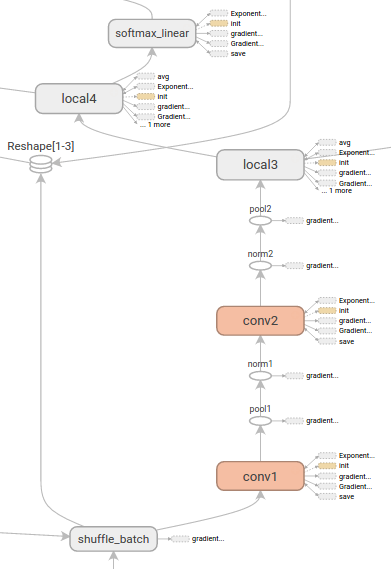
\includegraphics[width=0.5\textwidth]{hashtag_18}
    \bicaption{Tensorflow数据流动示意图}{Tensorflow data flow diagram}
    \label{fig:4_1}
\end{figure}

本文使用的是 Tensorflow1.6 ,根据官网的版本说明,Tensorflow 具有如下特 点:
\begin{enumerate}

\item \bfseries 性能最优化\mdseries 

由于 Tensorflow 给予了线程、队列、异步操作等以最佳的支持,Tensorflow 让你可以将你手边硬件的计算潜能全部发挥出来。你可以自由地将 Tensorflow图中的计算元素分配到不同设备上,Tensorflow 可以帮你管理好这些不同副本。

\item  \bfseries 灵活使用 \mdseries  

TensorFlow 不是一个严格的“神经网络”库。只要你可以将你的计算表示为 一个数据流图,你就可以使用 Tensorflow 来构建图,描写驱动计算的内部循环。 Tensorflow 提供了有用的工具来帮助你组装“子图”(常用于神经网络),当然用户 也可以自己在 Tensorflow 基础上写自己的“上层库”。定义顺手好用的新复合操作 和写一个 python 函数一样容易,而且也不用担心性能损耗。当然万一你发现找 不到想要的底层数据操作,你也可以自己写一点 c++ 代码来丰富底层的操作。

\item   \bfseries 高效开发\mdseries 

TensorFlow 保证了 Python API 稳定性,可以在不破坏现有的代码基础上获 取新功能。

\end{enumerate}

综上所述,Tensorflow 的出现大大方便了深度学习研究者们快速实现部署自 己的模型,用于机器学习和深度神经网络方面的研究。本章的模型部署在 Ten- sorflow 上,使用 GPU 加速训练,在模型训练阶段,使用随机梯度下降算法,在 整个实验过程中,本文观察到大概训练时间只需 3 个小时左右,模型就在训练数 据上收敛了。


\section{实验结果及分析}

\subsection{实验数据}
本章从微观角度刻画 Hashtag 流行度预测,将 Hashtag 的观测范围限定到一 小时内,然后预测二十四小时后的流行度。对于用到的用户粉丝网络结构数据依 然采取第三章的数据,其他数据如下。

用于提取 Hashtag 的数据如下,一共四百三十万左右的 Hashtag 数据,从这 些数据中构建训练样本。
\begin{table}[H]
    \centering
    \footnotesize% fontsize
         \bicaption{多源头 Hashtag 数据}{Multi-source Hashtag data}
      \label{tab:multi_h}
    \setlength{\tabcolsep}{30pt}% column separation
    \renewcommand{\arraystretch}{1.2}%row space 
    \begin{tabular}{cccc}
        \hline
       编号& 属性& 属性值 \\
        1 & 文件大小 & 1.1G\\
        2 & Hashtag 的消息数量 & 4322622\\
        %\cline{2-9}% partial hline from column i to column j
        \hline
        
        	\hline
    \end{tabular}

\end{table}
从以上数据构建多源头 Hashtag 训练样本,样本总数一共六万三千左右,训 练样本和验证样本大概七比一。

\begin{table}[H]
    \centering
    \footnotesize% fontsize
         \bicaption{多源头 Hashtag 训练样本数据}{Multi-source Hashtag training sample data}
      \label{tab:sample_hashtag}
    \setlength{\tabcolsep}{30pt}% column separation
    \renewcommand{\arraystretch}{1.2}%row space 
    \begin{tabular}{cccc}
        \hline
        编号 & 属性 & 属性值\\
        1 & 文件大小& 150M\\
        2 &Hashtag 训练样本数目& 63487\\
        %\cline{2-9}% partial hline from column i to column j
        \hline
        
        	\hline
    \end{tabular}

\end{table}

\subsection{评价指标}
模型在训练数据上进行训练,然后在测试数据上进行验证。针对测试数据中
的每一个 Hashtag, 本文预测其未来的流行度,采用如下评价指标进行评估:

 MSLE(mean squared log error)公式如\ref{eq:msle}所示, 函数计算了一个对应平方对数 (二次)误差或损失的预估值风险度量, 由于 Hashtag 的分布呈现幂率分布,因此
通过 log 运算,该指标更加适合具有指数增长趋势的数据。 

 \begin{equation}\label{eq:msle}
 	MSLE = \frac{1}{N}~\sum_{t=1}^N~(\log{(observed_t + 1)} - \log{(predicted_t + 1)})^2
 \end{equation}
 
 mSLE(median squared log error)公式如\ref{eq:mmsle}所示,该函数有趣有趣,因为它的离群值很强. 通过取目标和预测之间的所有 sle 的中值来计算损失.
 
  \begin{equation}\label{eq:mmsle}
  	\begin{split}
       mSLE = median((\log{(observed_1 + 1)} - \log{(predicted_1 + 1)})^2,...,\\
      ( \log{(observed_N + 1)} - \log{(predicted_N + 1)})^2)
       \end{split}
  \end{equation}

\subsection{结果分析}
\subsubsection{参数设置}
深度学习模型的特点之一就是有很多参数需要调整,本模型也不例外,参 数主要分为两类,一类是模型参数,一类是训练参数。模型参数比如每一层的特 征维度,attention 的大小,user embedding 的大小等等;训练参数,比如学习率, batch 大小,dropout 等等,这些参数对于模型结果都会产生很大影响。

论文主要采用网格搜索方法寻找最优参数,既先固定其他参数,然后调整某 个参数到最优,依次类推,找到每一个参数的最优,模型所用到的主要参数,含 义以及最终值如表\ref{tab:model_1}所示。

\begin{table}[H]
    \centering
    \footnotesize% fontsize
     \bicaption{模型参数表}{Model parameter table}
      \label{tab:model_1}
    \setlength{\tabcolsep}{30pt}% column separation
    \renewcommand{\arraystretch}{1.2}%row space 
    \begin{tabular}{cccc}
        \hline
        \textbf{模型参数}&\textbf{ 含义}&\textbf{ 取值} \\
        %\cline{2-9}% partial hline from column i to column j
        \hline
        \textbf{user~embedding} & 用户向量维度&  100\\
       \textbf{ sequences} &序列长度 &1000 \\
     \textbf{   steps }& 序列个数& 30\\
       \textbf{ $U_{S}$ }&局部序列 attention 上下文向量 & stddev=0.01\\
       \textbf{ $U_{M}$}&全局 attention 上下文向量 & stddev=0.01 \\
\textbf{        Fully Connected Layer} & 全连接的初始值&  [-1,1]\\
        	\hline
    \end{tabular}
    
\end{table}


模型训练所用到的主要参数,含义以及最终值如表\ref{tab:model_2}所示。

\begin{table}[H]
    \centering
    \footnotesize% fontsize
         \bicaption{模型训练参数}{Model training parameters}
      \label{tab:model_2}
    \setlength{\tabcolsep}{30pt}% column separation
    \renewcommand{\arraystretch}{1.2}%row space 
    \begin{tabular}{ccc}
        \hline
       \textbf{ 训练参数} & \textbf{含义} & \textbf{取值}   \\
        %\cline{2-9}% partial hline from column i to column j
        \hline
        \textbf{alpha }& 学习率 & 0.005 \\
        \textbf{rate~ for~ embedding} &用户 embedding 的学习速率&0.0005 \\
       \textbf{ dropout} & 正则大小 &0.8 \\
        \textbf{batch ~size} & 每批的大小& 32 \\
      \textbf{  l2 }& 正则项大小
  &0.05\\
        	\hline
    \end{tabular}

\end{table}

在这里,本文发现参数的设置对模型效果影响比较大,合适的参数加上合理 的模型结构,加上正确的优化目标才能够使模型达到最优效果,这三者缺一不 可。

\subsubsection{模型间对比}
为了验证模型的有效性,本文所采用的对比模型主要包括如下几种:
\begin{enumerate}
\item Model1 首先通过 DeepHawkes 模型对 Hashtag 的每个源头的数据进行分 别预测,然后将预测的结果求和,这个是最基础直观的操作,作为基本的 baseline。
\item Model2 为了验证 attention 对于序列之间的权重的衡量,将 DeepHawkes 模型中的时间衰减影响换成 attention 机制,最后将预测的结果求和。
\item Model3 为了验证 attention 对于 Hashtag 不同源头之间的权重的衡量,将 DeepHawkes 模型每个源头的输出结合 attention 来作为整体的表达,然后进行整 体的预测。
\end{enumerate}


本文将基于多源头的 Hashtag 流行度预测模型,与以上三种模型进行试验对比,结果对比如表\ref{tab:model_r}所示。

\begin{table}[H]
    \centering
    \footnotesize% fontsize
         \bicaption{模型之间结果对比}{Comparison of results between models}
      \label{tab:model_r}
    \setlength{\tabcolsep}{30pt}% column separation
    \renewcommand{\arraystretch}{1.2}%row space 
    \begin{tabular}{ccc}
        \hline
        \textbf{Models }& \textbf{MSLE }&\textbf{ mSLE} \\
        %\cline{2-9}% partial hline from column i to column j
        \hline
	    \textbf{Model1} & 3.72 & 1.06\\
	    	    \textbf{Model2} & 3.64 & 1.02\\
	     \textbf{Model3} & 3.42 & 0.94\\
        \textbf{本模型} & 3.38 & 0.88\\
        	\hline
    \end{tabular}

\end{table}


根据实验结果,我们发现基于 attention 的多源头的 Hashtag 流行度预测模型 可以有效刻画 Hashtag 的传播机制,和单源头消息的流行度预测模型 DeepHakwes 相比,效果有了明显提升,MSLE 提升了 9\%,证明模型的有效性。并且通过 Model1 和 Model2 之间的对比,加入的序列间的 attention 确实对模型有一定的帮助,效 果提升不高,可能是因为时间衰减因素所占的比重较大,对整体的影响很重要。 另外通过源头的 attention,发现 model3 比 model1 的效果提升了很多,MSLE 提 升了 8\%, 验证了 attention 对于多源的有效刻画。

为了展示用户向量的初始化方式对于模型的整体效果以及计算性能的影响, 本文将通过用户向量随机初始化作为输入与通过 LINE 模型得到的用户向量表 示进行对比,结果展示如表\ref{tab:model_user}所示,通过实验可知,通过使用预训练的方式学 习到的用户向量表达,对于整体结果有一定的提升,因为通过模型学到的用户向 量表达,其实也是训练数据下的用户粉丝网络结构的缩影,学习到的一种局部表 达,通过使用 LINE 进行预训练得到用户的向量表达,更加全面的反映了用户之 间的关系,对于模型的预测提供了更加全面的参考,并且节约了用户向量学习的 时间,模型整体的计算时间大大减少, 时间效率提高了 30\% 左右,为以后模型的 优化以及性能的提升提供了参考方向。

\begin{table}[H]
    \centering
    \footnotesize% fontsize
         \bicaption{用户向量的初始化方式对比}{Comparison of user vector initialization methods}
      \label{tab:model_user}
    \setlength{\tabcolsep}{30pt}% column separation
    \renewcommand{\arraystretch}{1.2}%row space 
    \begin{tabular}{cccc}
        \hline
        \textbf{Models }& \textbf{MSLE }&\textbf{ mSLE} & \textbf{time}\\
        %\cline{2-9}% partial hline from column i to column j
        \hline
	    \textbf{本模型 + 随机初始化} & 3.44 & 0.95 & 13469s\\
        \textbf{本模型 +LINE} & 3.38 & 0.88 & 9546s\\
        	\hline
    \end{tabular}

\end{table}


\section{本章总结}

对于传统的基于特征的 Hashtag 流行度预测问题,需要人工构造复杂的特 征,并且无法建模 Hashtag 传播中的机制,无法理解其内部具体的传播过程;另 一方面基于神经网络的消息流行度预测问题虽然刻画了消息内部的传播机制, 但是它解决的是单源头问题,无法有效的处理多源头的 Hashtag, 并且内部的时 间衰减影响无法刻画每条传播途径的区别。因此本章提出了一种基于多源头的 Hashtag 流行度预测模型,通过深度学习自动学习特征,并且针对时间衰减效应 采用 attention 机制,来建模每条路径的影响,同时针对多源头 Hashtag 的传播, 采用 attention 建模每个源头的重要性,有效的将多个源头整合到一起,实现了多 源头的 Hashtag 流行度预测。之后,使用 Tensorflow 平台进行模型的训练,测试。 通过实验证明,与其他模型相比,本文提出的模型是有效的,与 DeepHawkes 模 型相比,MSLE 提升了 9.1\%。